\chapter{Techniques for Language Processing}
\label{chapt:NLP}
\section{Background}
Natural Language Processing (henceforth NLP) is the application of computer science to study, model and understand human languages using computers. Machine learning, a class of algorithms for fitting and predicting patterns in data, is a powerful technique, with many applicatings in NLP. This section explores approaches to representing journal articles in a quantitative manner using NLP.
\section{Bag of Words}
A simple approach to representing a document is a \emph{bag of words} model. The document is split into component words in an unordered set. The model computes the number of distinct words in a corpus of documents, $N$. It then assigns each document in the corpus an $N$ dimensional vector $\mathbf{v}$. If document $A$ contains word $i$ 2 times, then $v_{A, i } = 2$. A simple example is given below:

Document A: \texttt{A good yield was obtained for a nucleophile}

Document B: \texttt{The nucleophile is a good donor}
\begin{table}[H]
\label{tab:BAGOFWORDS}
\caption{Bag of words}
\begin{center}
\begin{tabular}{||c|c|c||}
\hline
Vocabulary &  $\mathbf{v}_A$ & $\mathbf{v}_B$\\
\hline
A & 2 & 1\\
Good & 1 & 1\\
Nucleophile & 1 & 1 \\
Yield & 1 & 0\\
For & 1& 0\\
Is & 0 & 1\\
The & 1 & 0\\
Donor & 0 & 1\\
Was & 1 & 0\\
\hline
\end{tabular}
\end{center}
\end{table}
Table \ref{tab:BAGOFWORDS} shows the vector representations for Documents A and B. The higher the scalar product of normalised $\mathbf{v}_A \cdot \mathbf{v}_A$, the more similar the documents are predicted to be. This model is used extensively in industry. A related model, the \emph{bag of citations} model sets vector components are the presence or absence of citations. Both models are widely used in industry for analysing the publishing landscape.
\section{Word2Vec}
\label{sec:WORD2VEC}
The \emph{Bag of Words} model treats words as atomic units, beneficial for robust and fast computation. However, words can have degrees of similarity to each other, and these relationships are not captured by bag of words models \cite{word2veckingqueen}. Distributed representations of words have been used to address this for some time \cite{distributedrepresentations}.

 A recent successful approach has been the Word2Vec algorithm \cite{word2vec1} \cite{word2vec2}. The Word2Vec algorithm uses a neural net to represent words as vectors in a continuous rather than discrete space. Vectors for words with similar meanings will point in similar directions in this `Semantic space'.The Word2Vec algorithm is fed a language corpus sentence by sentence. The words within the sentences have a semantic relationship, which the algorithm uses to infer word meanings. 
 
This is achieved with two architectures, Continuous Bag of Words (henceforth CBOW) and skip-gram. The CBOW architecture uses a shallow neural net to predict a word's vector by summing or averaging the vectors of the surrounding words in a training sentence. The skip-gram algorithm predicts the vectors of words surrounding the current training word. By training with many input sentences, prediction vectors are gradually improved. 

\begin{figure}[H]
    \centering
    \textbf{Word2Vec architectures}\par\medskip
    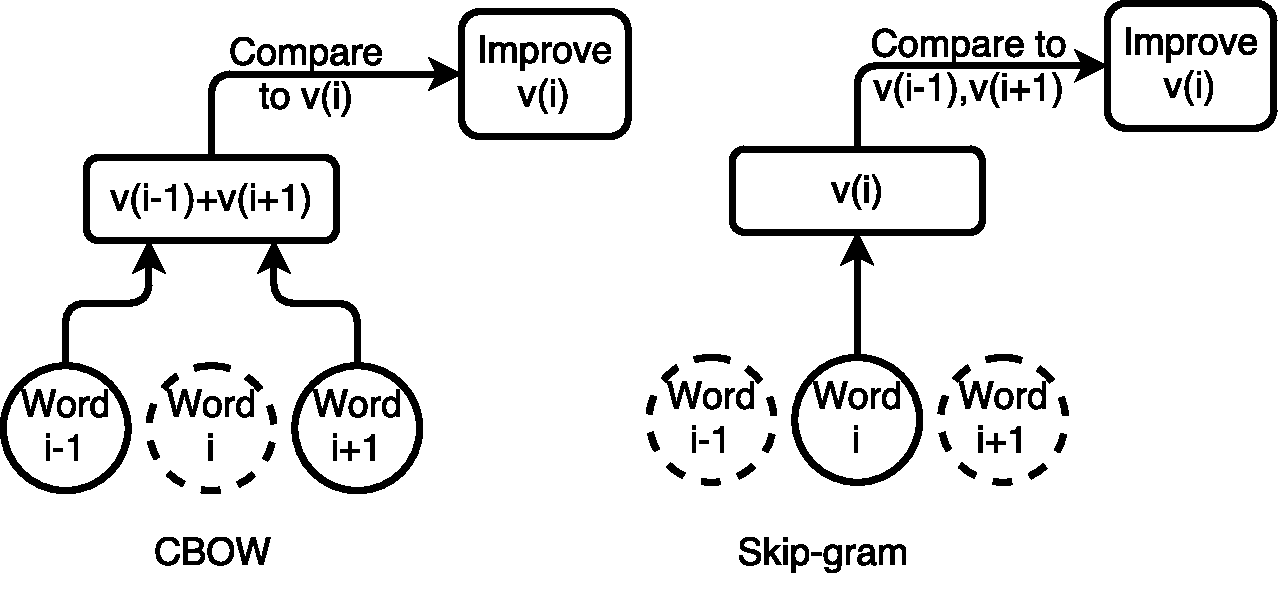
\includegraphics[width=\textwidth]{Natural_Language_Processing/cbow_v_skip.pdf}
    \caption{The training architectures of the Word2Vec training algorithm. Word vectors are denoted $v(i)$ for word i. In CBOW word i is predicted by the vector found by summing vectors surrounding i, and $v(i)$ is adjusted to be closer to this prediction. In skip-gram, word i's vector is pairwise compared to its context words, here i-1 and i+1 as a basis to improve $v(i)$.). CBOW attemtps to make words similar the sum of the surrounding words, skipgram attempts to minimise distance to each surrounding word.}
     \label{fig:CBOWSKIP}
\end{figure}

The training process is shown in figure \ref{fig:CBOWSKIP}. CBOW uses a fixed window of words surrounding the current training word. The order of words within the window does not matter, but because the window `slides' along as the algorithm considers words i+1, i+2... word ordering is represented in the model . In skip-gram, a random number of nearby words are used for the prediction vectors for word i. 

The model has added sophistication built in to reduce the importance of very commonly occurring words, and to identify phrases. The word vectors that are produced encapsulate both semantic and syntactic meanings and can be manipulated to represent concepts and relationships.
\begin{figure}[H]
    \centering
    \textbf{Word Vector Relationships}\par\medskip
    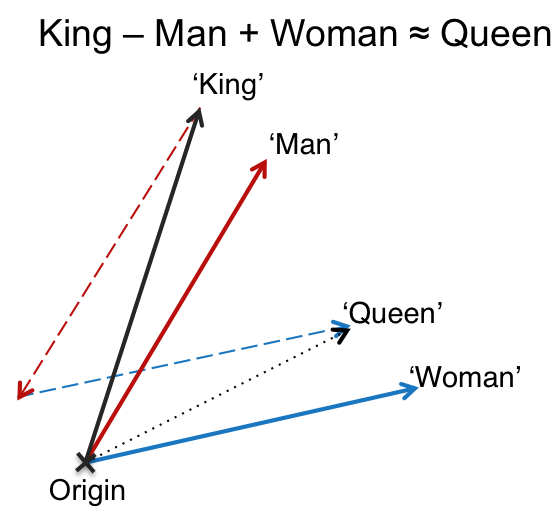
\includegraphics[height=6.5cm]{Natural_Language_Processing/KINGQUEEN.png}
    \caption{Schematic Representation of how concepts can be represented in word vector space. Word2Vec is able to replicate this behaviour. The vector found by vec(‘King’)- vec(‘Man’)+vec(‘Woman’) is approximately equal to vec(‘Queen’). The model has been tested on thousands of similar examples\cite{word2vec2}\cite{word2veckingqueen}.}
     \label{fig:KINGQUEEN}
\end{figure}
Word2Vec models are able to represent concepts by vector algebraic operations on their word representations. Figure \ref{fig:KINGQUEEN} shows one famous example a Word2Vec model trained on the `Google News' text corpus was able to identify. 

\section{Doc2Vec}
The Doc2Vec algorithm \cite{gensim}(an implementation of Paragraph Vectors \cite{doc2vec}) allows the Word2vec process to directly learn vectors that represent documents. The CBOW model is adapted so that, in addition to word vectors, each document is associated with its own vector that contributes to the vector sum predictions in training. The result is that an entire document can be represented by a vector in a document semantic space.

The nature of the collected metadata detailed in \S\ref{chapt:DATA_ACQUISITION} lends itself naturally to the Word2Vec and Doc2Vec algorithms, as it is a large store of natural language, rich with encoded information. The focus of the machine learning analysis phase of the project was directed at applying the Word2Vec and Doc2Vec algorithms to the dataset to try and automatically learn and classify chemical semantic concepts. These investigations are detailed in the following sections.